% Created 2021-08-13 Fri 15:28
% Intended LaTeX compiler: pdflatex
\documentclass[11pt]{article}
\usepackage[utf8]{inputenc}
\usepackage[T1]{fontenc}
\usepackage{graphicx}
\usepackage{grffile}
\usepackage{longtable}
\usepackage{wrapfig}
\usepackage{rotating}
\usepackage[normalem]{ulem}
\usepackage{amsmath}
\usepackage{textcomp}
\usepackage{amssymb}
\usepackage{capt-of}
\usepackage{hyperref}
\author{Sreejith Sreekumar}
\date{\today}
\title{Generating initial feature set}
\hypersetup{
 pdfauthor={Sreejith Sreekumar},
 pdftitle={Generating initial feature set},
 pdfkeywords={},
 pdfsubject={},
 pdfcreator={Emacs 26.3 (Org mode 9.1.9)}, 
 pdflang={English}}
\begin{document}

\maketitle
\tableofcontents


\section{Features}
\label{sec:org64cc0d5}

\begin{enumerate}
\item Simple Moving Average
\begin{itemize}
\item Usual shift periods used are 14, 50 and 200
\end{itemize}
\item Relative Strength Index
\end{enumerate}

\begin{equation}
     Relative Strength, RS = \frac{Average\ Gain\ Over\ n\ periods}{Average\ Loss\ Over\ n\ periods}
\end{equation}
\begin{equation}
     RSI = 100 - \frac{100}{1 + RS}
\end{equation}


\begin{verbatim}

feature_names = ['5d_close_pct']  # a list of the feature names for later

# Create moving averages and rsi for timeperiods of 14, 30, 50, and 200
for n in [14, 30, 50, 200]:

    # Create the moving average indicator and divide by Adj_Close
    lng_df['ma' + str(n)] = talib.SMA(lng_df['Adj_Close'].values,
                              timeperiod=n) / lng_df["Adj_Close"]
    # Create the RSI indicator
    lng_df['rsi' + str(n)] = talib.RSI(lng_df['Adj_Close'].values, timeperiod=n)

    # Add rsi and moving average to the feature name list
    feature_names = feature_names + ['ma' + str(n), 'rsi' + str(n)]

print(feature_names)



# Drop all na values
lng_df = lng_df.dropna()

# Create features and targets
# use feature_names for features; '5d_close_future_pct' for targets
features = lng_df[feature_names]
targets = lng_df["5d_close_future_pct"]

# Create DataFrame from target column and feature columns
feature_and_target_cols = ['5d_close_future_pct'] + feature_names
feat_targ_df = lng_df[feature_and_target_cols]

# Calculate correlation matrix
corr = feat_targ_df.corr()
print(corr)



# Plot heatmap of correlation matrix
sns.heatmap(corr, annot= True, annot_kws = {"size": 14})
plt.yticks(rotation=0, size = 14); plt.xticks(rotation=90, size = 14)  # fix ticklabel directions and size
plt.tight_layout()  # fits plot area to the plot, "tightly"
plt.show()  # show the plot


\end{verbatim}



\begin{center}
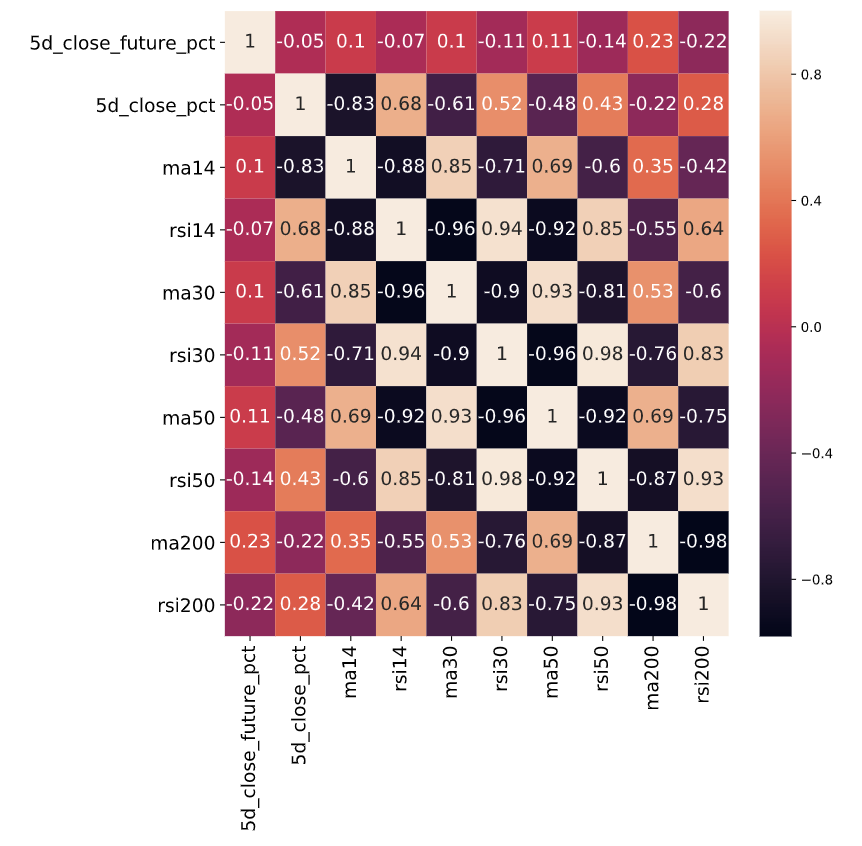
\includegraphics[width=.9\linewidth]{corr.png}
\end{center}
\end{document}